\subsubsection{Networks}

So far, we have described the internal structure of \textbf{one LSTM cell}. But real sequence tasks require using this cell \textbf{repeatedly, one timestep at a time}. Thus, an \important{LSTM network} is simply \textbf{a chain of identical LSTM cells, each processing one element of the sequence, sharing all parameters}. With ``identical'', we mean that all cells have the same weights, same biases, same gates, and same equations. Only the \textbf{inputs} $x_t$ and \textbf{internal states} $\left(h_t, C_t\right)$ differ from cell to cell, depending on the timestep $t$.

\highspace
The LSTM \textbf{unrolled across timesteps}:
\begin{itemize}
    \item $x_1, x_2, \ldots, x_T$ are the inputs at each timestep;
    \item At each timestep $t$, the LSTM cell receives \textbf{current input} $x_t$ and \textbf{previous states} $\left(h_{t-1}, C_{t-1}\right)$;
    \item It computes \textbf{new hidden state} $h_t$, \textbf{new cell state} $C_t$ using the same equations, weights, and biases at each timestep, and produces \textbf{output} $y_t$ (if relevant).
\end{itemize}
The key idea is \textbf{all cells share parameters, but each has its own internal states as time progresses}. This allows the network to \textbf{learn temporal patterns} in the data, as information can flow through the cell states across many timesteps, while the shared parameters ensure consistency in how information is processed at each step.

\begin{figure}[!htp]
    \centering
    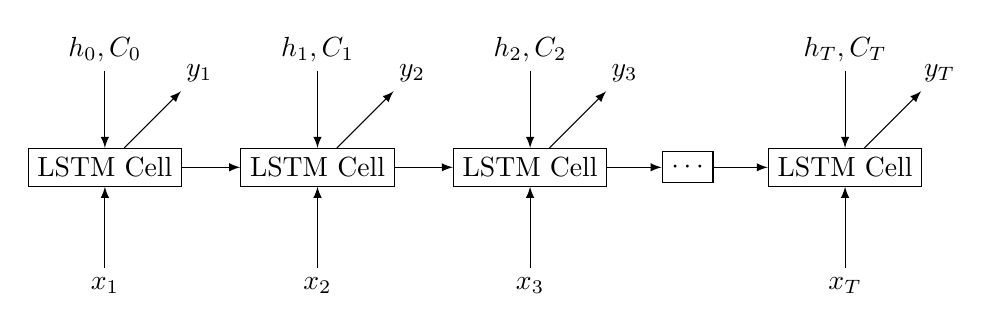
\begin{tikzpicture}[node distance=2cm, auto, >=latex]
        % Nodes
        \node[draw, rectangle] (lstm1) {LSTM Cell};
        \node[draw, rectangle, right of=lstm1, node distance=2.7cm] (lstm2) {LSTM Cell};
        \node[draw, rectangle, right of=lstm2, node distance=2.7cm] (lstm3) {LSTM Cell};
        \node[draw, rectangle, right of=lstm3, node distance=2cm] (dots) {$\cdots$};
        \node[draw, rectangle, right of=dots,  node distance=2cm] (lstmT) {LSTM Cell};
        \node[below of=lstm1, node distance=1.5cm] (x1) {$x_1$};
        \node[below of=lstm2, node distance=1.5cm] (x2) {$x_2$};
        \node[below of=lstm3, node distance=1.5cm] (x3) {$x_3$};
        \node[below of=lstmT, node distance=1.5cm] (xT) {$x_T$};
        \node[above of=lstm1, node distance=1.5cm] (h0) {$h_0, C_0$};
        \node[above of=lstm2, node distance=1.5cm] (h1) {$h_1, C_1$};
        \node[above of=lstm3, node distance=1.5cm] (h2) {$h_2, C_2$};
        \node[above of=lstmT, node distance=1.5cm] (hT) {$h_T, C_T$};
        % Output nodes
        \node[right of=lstm1, node distance=0.8cm, above of=lstm1, node distance=1.2cm] (y1) {$y_1$};
        \node[right of=lstm2, node distance=0.8cm, above of=lstm2, node distance=1.2cm] (y2) {$y_2$};
        \node[right of=lstm3, node distance=0.8cm, above of=lstm3, node distance=1.2cm] (y3) {$y_3$};
        \node[right of=lstmT, node distance=0.8cm, above of=lstmT, node distance=1.2cm] (yT) {$y_T$};
        % Arrows
        \draw[->] (x1) -- (lstm1);
        \draw[->] (x2) -- (lstm2);
        \draw[->] (x3) -- (lstm3);
        \draw[->] (xT) -- (lstmT);
        \draw[->] (h0) -- (lstm1);
        \draw[->] (h1) -- (lstm2);
        \draw[->] (h2) -- (lstm3);
        \draw[->] (hT) -- (lstmT);
        \draw[->] (lstm1) -- (lstm2);
        \draw[->] (lstm2) -- (lstm3);
        \draw[->] (lstm3) -- (dots);
        \draw[->] (dots) -- (lstmT);
        % Output arrows
        \draw[->] (lstm1) -- (y1);
        \draw[->] (lstm2) -- (y2);
        \draw[->] (lstm3) -- (y3);
        \draw[->] (lstmT) -- (yT);
    \end{tikzpicture}
    \captionof{figure}{\textbf{LSTM network} (many-to-many architecture) \textbf{unrolled across timesteps}. Each LSTM cell processes one input at a time, sharing parameters but maintaining its own internal states. Outputs can be produced at each timestep if required.}
    \label{fig:lstm-unrolled-many-to-many}
\end{figure}

\begin{flushleft}
    \textcolor{Green3}{\faIcon{question-circle} \textbf{What does the LSTM actually learn over time?}}
\end{flushleft}
As it processes a sequence, the LSTM network \textbf{learns to update its cell state} $C_t$ and \textbf{hidden state} $h_t$ in a way that captures relevant information from the inputs over time. The LSTM network:
\begin{itemize}
    \item[\textcolor{Green3}{\faIcon{check}}] \textbf{Accumulates information in the cell state}. This allows it to remember important features of the input sequence over long periods.
    \item[\textcolor{Green3}{\faIcon{check}}] \textbf{Selective memory updates}. Updates memory only when needed. The gates control when to forget old information and when to add new information, enabling the network to focus on relevant parts of the sequence.
    \item[\textcolor{Green3}{\faIcon{check}}] \textbf{Outputs predictions for each step}. The hidden state $h_t$ can be used to make predictions at each timestep, allowing the network to generate outputs based on the learned temporal patterns.
    \item[\textcolor{Green3}{\faIcon{check}}] \textbf{Adapts context dynamically}. The LSTM can adjust its memory based on the context of the sequence, making it effective for tasks like language modeling, time series prediction, and more.
\end{itemize}
These capabilities allow LSTM networks to understand temporal relationships (e.g., sequences in text, speech, or time series data), dependencies across distant timesteps (e.g., long-term dependencies in sentences), evolving contexts (e.g., changing topics in a conversation), and patterns different lengths (e.g., variable-length sequences in natural language).

\highspace
\begin{flushleft}
    \textcolor{Green3}{\faIcon{question-circle} \textbf{How LSTMs are used in real models}}
\end{flushleft}
LSTMs can be arranged in different \textbf{architectural patterns} depending on the task. Each \hl{pattern corresponds to how inputs and outputs are handled across time}. These patterns apply not only to LSTMs, but also to GRUs, Transformers, and any sequential model. However, LSTMs are particularly well-suited for these patterns due to their ability to manage long-term dependencies. The main patterns are:
\begin{enumerate}
    \item \important{Many-to-Many (Sequence-to-Sequence Output)}. \textbf{Output produced at \emph{each} timestep}. This is the architecture shown on \autoref{fig:lstm-unrolled-many-to-many}; each LSTM cell processes a timestep and emits an output:
    \begin{equation*}
        \left(x_{1} \to h_{1} \to y_{1}\right), \quad \left(x_{2} \to h_{2} \to y_{2}\right), \quad \ldots, \quad \left(x_{T} \to h_{T} \to y_{T}\right)
    \end{equation*}
    \textcolor{Green3}{\faIcon{question-circle} \textbf{When is this used?}}
    \begin{itemize}
        \item \textbf{Part-of-Speech tagging}: Assigning a part of speech to each word in a sentence.
        \item \textbf{Named Entity Recognition (NER)}: Identifying entities (like\break names, locations) in text.
        \item \textbf{Frame-by-frame video classification}: Classifying each frame in a video sequence.
        \item \textbf{Time-series forecasting}: Predicting future values at each time step.
        \item \textbf{Speech recognition}: Transcribing spoken words into text in real-time.
    \end{itemize}
    In this model, the input sequence and output sequence are of the same length, with each input element corresponding to an output element. For example, if the input is ``John likes cats'', the output could be ``Noun Verb Noun'' for part-of-speech tagging.


    \item \important{Many-to-One (Sequence Classification)}. \textbf{Use the \emph{final hidden state} $h_T$ to classify the entire sequence}. The architecture looks like this:
    \begin{equation*}
        h_{T} = \text{LSTM}\left(x_1, x_2, \ldots, x_T\right)
    \end{equation*}
    \begin{equation*}
        y = \text{softmax}\left(W h_T + b\right)
    \end{equation*}
    \textcolor{Green3}{\faIcon{question-circle} \textbf{When is this used?}}
    \begin{itemize}
        \item \textbf{Sentiment analysis}: Classifying the sentiment of a movie review (positive/negative).
        \item \textbf{Sequence classification}: Classifying DNA sequences or protein sequences.
        \item \textbf{Spam detection}: Classifying emails or messages as spam or not spam.
        \item \textbf{Audio classification}: Classifying audio clips into categories (e.g., music genre).
    \end{itemize}
    Here, the entire input sequence is summarized into a single vector (the final hidden state), which is then used for classification. For example, given a movie review, the model predicts whether the sentiment is positive or negative based on the entire text: ``The movie was fantastic!'' $\to$ ``Positive''. So, the \textbf{model uses \emph{all} the timesteps} but \textbf{only the \emph{final} state matter for classification}.


    \item \important{One-to-Many (Sequence Generation / Decoder)}. \textbf{Start from a single input and generate a sequence}. For example:
    \begin{equation*}
        h_{0} = f(x) \quad \text{(embedding of a single input)}
    \end{equation*}
    \begin{equation*}
        y_1, y_2, \ldots, y_T = \text{LSTM}\left(h_0\right)
    \end{equation*}
    This is typically autoregressive:
    \begin{itemize}
        \item At step 1, input $h_0$ produces output $y_1$;
        \item At step 2, input is $y_1$ (or its embedding), producing $y_2$;
        \item This continues until the full sequence is generated.
    \end{itemize}
    \textcolor{Green3}{\faIcon{question-circle} \textbf{When is this used?}}
    \begin{itemize}
        \item \textbf{Text generation}: Generating sentences or paragraphs from a\break prompt.
        \item \textbf{Image captioning}: Generating a descriptive caption for an image.
        \item \textbf{Music generation}: Composing music sequences from a seed note or chord.
        \item \textbf{Auto-regressive generation}: Generating sequences in tasks like language modeling.
    \end{itemize}
    Here, the \textbf{model starts with a single input} (like a prompt or seed, a vector) and \textbf{generates a sequence of outputs step by step}. For example, given the prompt ``Once upon a time'', the model might generate a full story.


    \item \important{Encoder-Decoder (Seq2Seq) Architecture}. \textbf{Use one LSTM (encoder) to process the input sequence into a context vector, then another LSTM (decoder) to generate the output sequence from that vector}. This pattern is still used in modern Transformers. It is a \textbf{two-part LSTM system}:
    \begin{enumerate}
        \item \textbf{Encoder}: Processes the input sequence $\left(x_1, x_2, \ldots, x_T\right)$ and produces a context vector (final hidden state) $h_T$:
        \begin{equation*}
            h_{T} = \text{LSTM}_{\text{enc}}\left(x_1, x_2, \ldots, x_T\right)
        \end{equation*}
        \item \textbf{Decoder}: Takes the context vector $h_T$ and generates the output sequence $\left(y_1, y_2, \ldots, y_{K}\right)$:
        \begin{equation*}
            y_1, y_2, \ldots, y_{K} = \text{LSTM}_{\text{dec}}\left(h_T\right)
        \end{equation*}
    \end{enumerate}
    \textcolor{Green3}{\faIcon{question-circle} \textbf{When is this used?}}
    \begin{itemize}
        \item \textbf{Machine translation}: Translating sentences from one language to another (e.g., English to French).
        \item \textbf{Dialogue systems}: Generating responses in chatbots.
        \item \textbf{Summarization}: Creating concise summaries of longer texts.
        \item \textbf{Speech-to-text}: Converting spoken language into written text.
        \item \textbf{Question answering}: Generating answers based on a given context or passage.
        \item \textbf{Autoencoders for sequences}: Learning compressed representations of sequences.
    \end{itemize}
    Here, the \textbf{input and output sequences can have different lengths}. For example, translating ``I love programming'' (3 words) to ``J'adore la programmation'' (4 words). The encoder captures the meaning of the input sequence, and the decoder generates the corresponding output sequence.


    \item \important{Many-to-Many with Different Lengths (e.g., CTC, translation)}. \textbf{Input and output sequences have different lengths, with outputs produced at each timestep}. This is common in tasks like speech recognition or translation where the number of input timesteps does not match the number of output timesteps. The architecture looks like this:
    \begin{equation*}
        y_1, y_2, \ldots, y_{K} = \text{LSTM}\left(x_1, x_2, \ldots, x_T\right)
    \end{equation*}
    \textcolor{Green3}{\faIcon{question-circle} \textbf{When is this used?}}
    \begin{itemize}
        \item \textbf{Speech recognition}: Converting audio signals into text, where the number of audio frames may differ from the number of words.
        \item \textbf{Machine translation}: Translating sentences where the source and target languages have different word counts.
        \item \textbf{Handwriting recognition}: Recognizing handwritten text from images, where the number of strokes may differ from the number of characters.
    \end{itemize}
    Here, the model processes the entire input sequence and produces an output sequence that may be of different length. Techniques like Connectionist Temporal Classification (CTC) are often used to align the input and output sequences during training.
\end{enumerate}
LSTMs are flexible enough to be used in almost every sequential modeling configuration. Their structure allows handling variable-length sequences, producing or consuming sequences, compressing long contexts, and dynamically generating outputs based on learned temporal patterns.